We were primarily interested in two major results produced in \cite{Fiete}. First, we were interested the occurrence of long synfire chains with synchronous regular firing. We also investigated the paper's claim that STDP learning with \(w_{max} = W_{max}\) converged to scaled permutation matrices.

Though we tried to replicate the algorithm described in \cite{Fiete}, we were unable to produce a stable system with the provided inputs, so we had to tune the parameters a bit. We eventually found parameters at which burst rates were steady and believable. 

With the parameters we found, we were able to observe weaker versions of most of the observations in the paper. We found that weight matrices converged near permutation matrices and we were able to observe some short sequences of firing chains, but we did not see the synchronous regular behavior exhibited in the paper.

Finally, we replaced STDP learning with Hebbian learning and demonstrated that the weights of a system undergoing Hebbian learning with soft and hard limits converged as closely or better to permutation matrices than they did under STDP learning.

\subsection{Parameter Tuning}

Although our model was constructed to be identical to the model used in \cite{Fiete}, we were unable to use the same parameters as the paper. As an example, the paper claimed to set \(r_{in}\), external input, at 4 Hz. At 4 Hz, we were unable to get our system to fire at all! We assumed it was a typo (the rest of the parameters were given in terms of ms), and attempted running our simulation at 4000Hz. Even 4000Hz was not enough to get the system started, so we tried simulated annealing. The system began with 10000Hz of stimulation, which decreased steadily to 4000Hz. We did this again, but this time stopped at 6000Hz. The difference was striking (see figure \ref{burstSTDP}). 

\begin{figure}[H]
\centering
\begin{subfigure}[b]{0.49\textwidth}
\includegraphics[width=\textwidth]{Burst_plot_4000Hz.eps}
\caption{4000 Hz}
\label{burstSTDP:4000}
\end{subfigure}
\,
\begin{subfigure}[b]{0.49\textwidth}
\includegraphics[width=\textwidth]{Burst_plot_6000Hz.eps}
\caption{6000 Hz}
\label{burstSTDP:6000}
\end{subfigure}
\caption{In figure 4 of \cite{Fiete}, the authors displayed a burst plot in which each neuron burst every 75 ms with high synchrony and regularity. We did not observe such synchrony in either plot, but the average frequency of firing in (b) was approximately 75 ms. Notice both systems exhibited exaggerated firing in the beginning. This was a consequence of simulated annealing.}
\label{burstSTDP}
\end{figure}

Beside \(r_{in}\), we spent a lot of time finding appropriate values for \(\eta\) and \(\epsilon\). 

\(\eta\) is the learning step-size. If \(\eta\) is too small, the weight matrix will not converge in a reasonable amount of time. If it is too large, whenever the weight matrix overshoots the soft limit, it will do so by a large margin, which will prompt large corrective measures, so convergence to a permutation matrix (which is barely under the soft limit), will not be plausible.
 
\(\epsilon\) is the strength of the soft limit. If \(\epsilon\) is too small, then when the weight matrix passes the soft limit it will not experience very strong hLTD. This will have the effect of weakening heterosynaptic competition. If \(\epsilon\) is too large, then each time the weight matrix passes the soft limit, it will experience very strong hLTD. Because the permutation matrix is on the border of the soft limit, having a large \(\epsilon\) will make any permutation matrix an unstable critical point in our simulation.

To evaluate these, we ran the simulation on a large combination of parameter values for \(r_{in}, \eta\) and \(\epsilon\). For each of these, we tested convergence using an error function (see section 3.2). The results are shown below:

\begin{figure}[H]
\centering
\begin{subfigure}[b]{0.49\textwidth}
\includegraphics[width = \textwidth]{Error_Scatter_all.eps}
\label{Error_scatter: all}
\caption{Errors of all simulations run}
\end{subfigure}
\,
\begin{subfigure}[b]{0.49\textwidth}
\includegraphics[width = \textwidth]{Error_Scatter_constantproduct.eps}
\label{Error_scatter: constant product}
\caption{Scatterplot of all errors with constant product}
\end{subfigure}
\label{Error_scatter}
\caption{Compare the two}
\end{figure}

Setting \(w_{max}\). (Burst History)

\begin{figure}[H]
\centering
\begin{subfigure}[b]{0.49\textwidth}
\includegraphics[width = \textwidth]{Burst_nolearning_perm_6000Hz_wmax0.14.eps}
\label{Burst_no_learning: 0.14}
\caption{Bursts without learning, \(w_max = 0.14\).}
\end{subfigure}
\,
\begin{subfigure}[b]{0.49\textwidth}
\includegraphics[width = \textwidth]{Burst_nolearning_perm_6000Hz_wmax0.3.eps}
\label{Burst_no_learning: 0.3}
\caption{Bursts without learning, \(w_max = 0.3\).}
\end{subfigure}
\\
\begin{subfigure}[b]{0.49\textwidth}
\includegraphics[width = \textwidth]{Burst_nolearning_perm_6000Hz_wmax0.5.eps}
\label{Burst_no_learning: 0.5}
\caption{Bursts without learning, \(w_max = 0.5\).}
\end{subfigure}
\,
\begin{subfigure}[b]{0.49\textwidth}
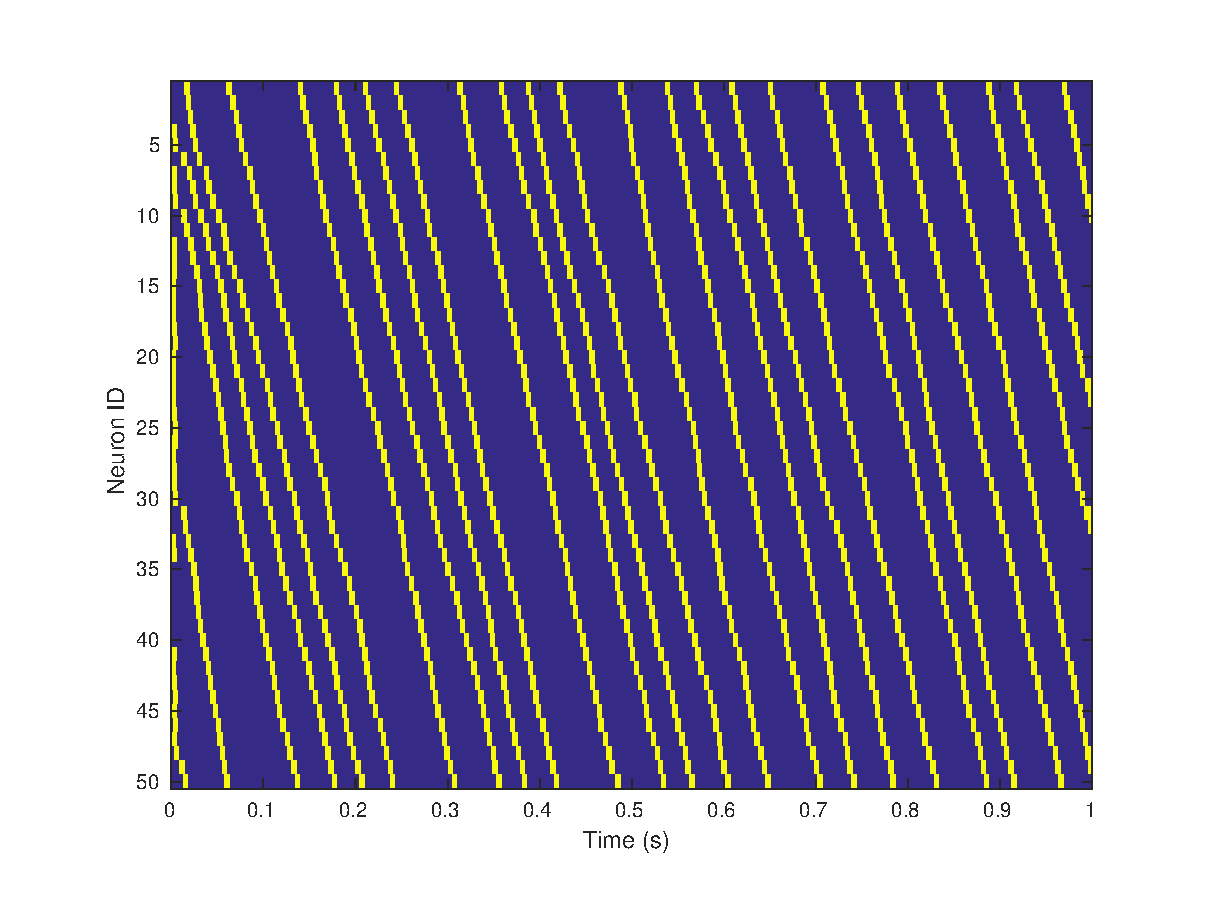
\includegraphics[width = \textwidth]{Burst_nolearning_perm_6000Hz_wmax0.7.eps}
\label{Burst_no_learning: 0.7}
\caption{Bursts without learning, \(w_max = 0.7\).}
\end{subfigure}
\label{Burst_no_learning}
\caption{Compare the four}
\end{figure}


\subsection{Convergence and Stability}

\begin{itemize}
\item Demonstrate the stability of our IB model by showing the firing rate plot and how it splits according to \(r_{in}\).

\begin{figure}[H]
\centering
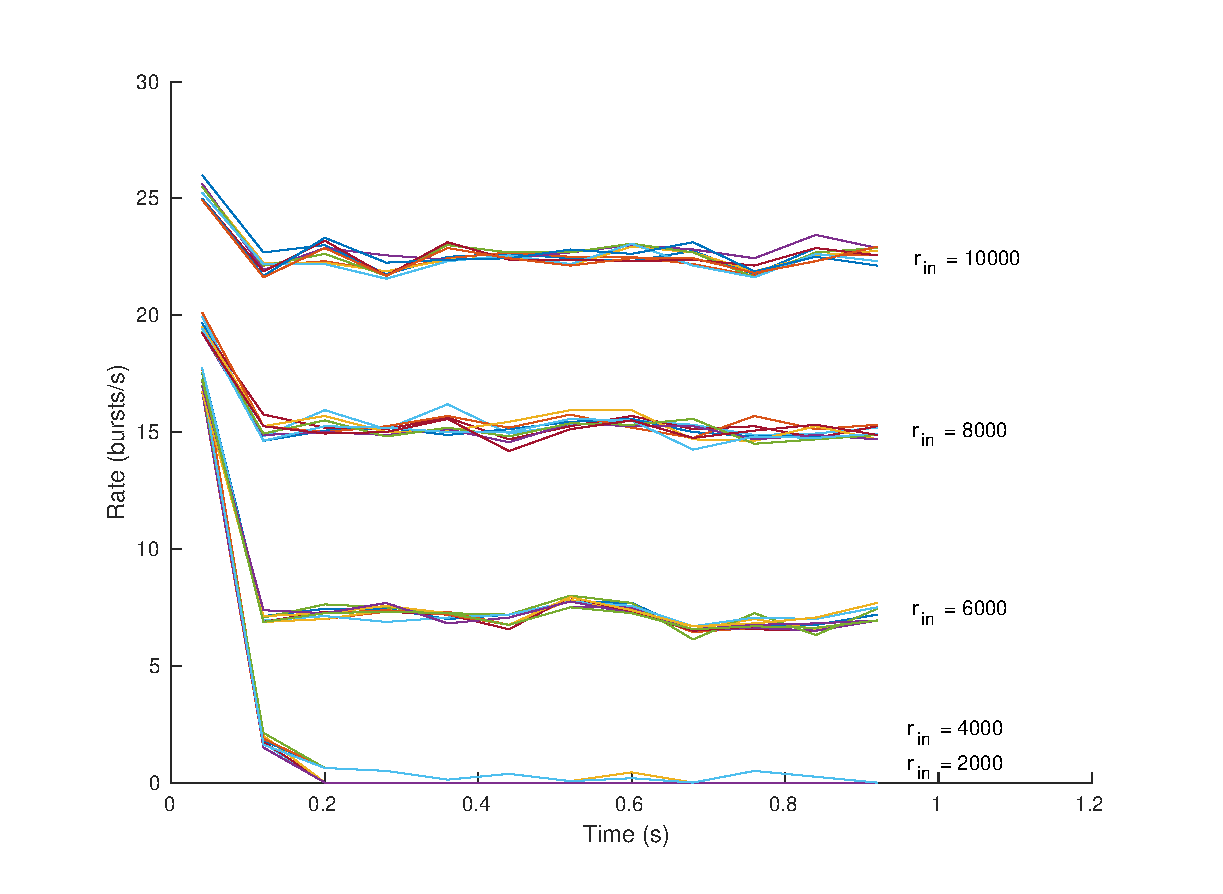
\includegraphics[scale = 0.4]{Firing_Rate_Binsize_80ms.eps}
\label{FR}
\caption{Caption will go here}
\end{figure}

\item Plot Weight and \(WW^T\) for 4000 and 6000 Hz to show some level of convergence.

\begin{figure}[H]
\centering
\begin{subfigure}[b]{0.49\textwidth}
\includegraphics[width = \textwidth]{Weights_4000Hz.eps}
\label{Weights: 4000Hz, basic}
\caption{Weight matrix of 4000Hz annealed}
\end{subfigure}
\,
\begin{subfigure}[b]{0.49\textwidth}
\includegraphics[width = \textwidth]{Weights_6000Hz.eps}
\label{Weights: 6000Hz, basic}
\caption{Weight matrix of 6000Hz annealed}
\end{subfigure}
\\
\begin{subfigure}[b]{0.49\textwidth}
\includegraphics[width = \textwidth]{WW_4000Hz.eps}
\label{Weights: 4000Hz, product}
\caption{\(WW^T\) of 4000Hz annealed}
\end{subfigure}
\,
\begin{subfigure}[b]{0.49\textwidth}
\includegraphics[width = \textwidth]{WW_6000Hz.eps}
\label{Weights: 6000Hz, product}
\caption{\(WW^T\) of 6000Hz annealed}
\end{subfigure}
\label{Weights}
\caption{Compare the four}
\end{figure}

\item Plot error function over time from normal and from permutation matrix

\begin{figure}[H]
\centering
\begin{subfigure}[b]{0.49\textwidth}
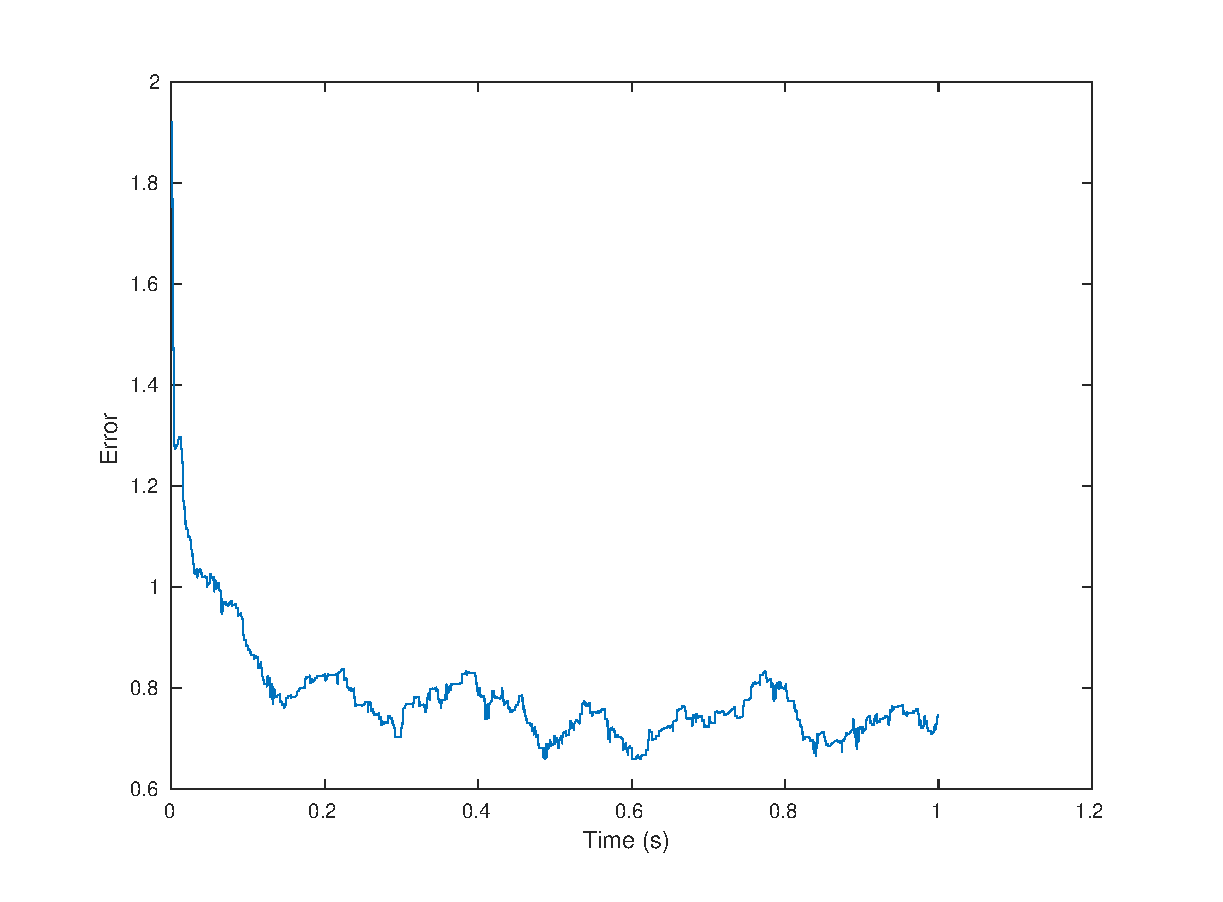
\includegraphics[width = \textwidth]{ErrorOverTime_6000Hz_normal.eps}
\label{Error_over_time: normal}
\caption{Plot of error in weights over time starting from a full connection weight matrix.}
\end{subfigure}
\,
\begin{subfigure}[b]{0.49\textwidth}
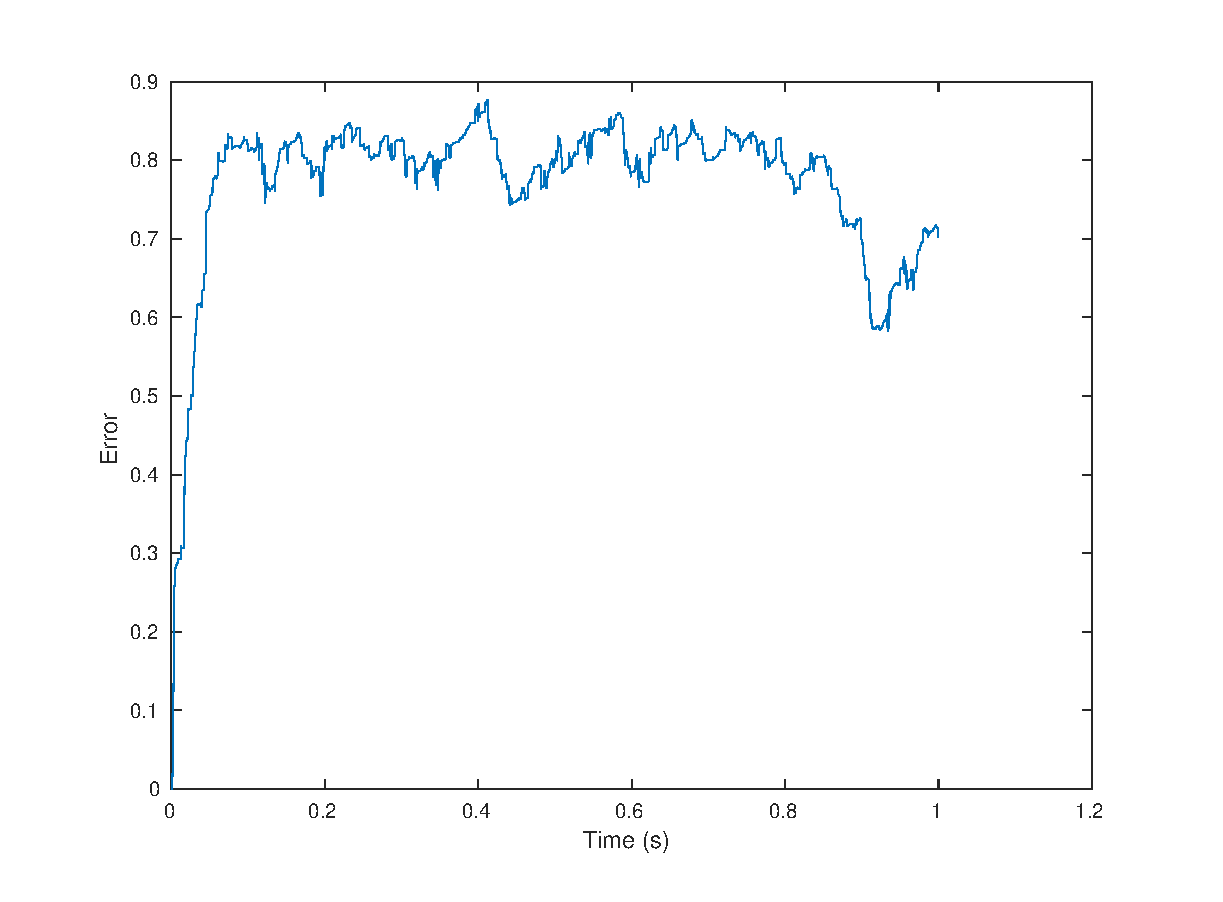
\includegraphics[width = \textwidth]{ErrorOverTime_6000Hz_Perm.eps}
\label{Error_over_time: permutation}
\caption{Plot of error in weights over time starting from a permutation weight matrix.}
\end{subfigure}
\label{Error_over_time}
\caption{Compare the two}
\end{figure}

\item Describe why the error function converges away from (mistake, see discussion).
\end{itemize}

\subsection{Hebbian Learning versus STDP}

\begin{itemize}
\item Introduce the idea of the refutation. 
\item Give a theoretical description why the type of learning should be relatively unimportant.
\item Compare plots (\(WW^T\), Error vs Time, Burst History).

\begin{figure}[H]
\centering
\begin{subfigure}[b]{0.49\textwidth}
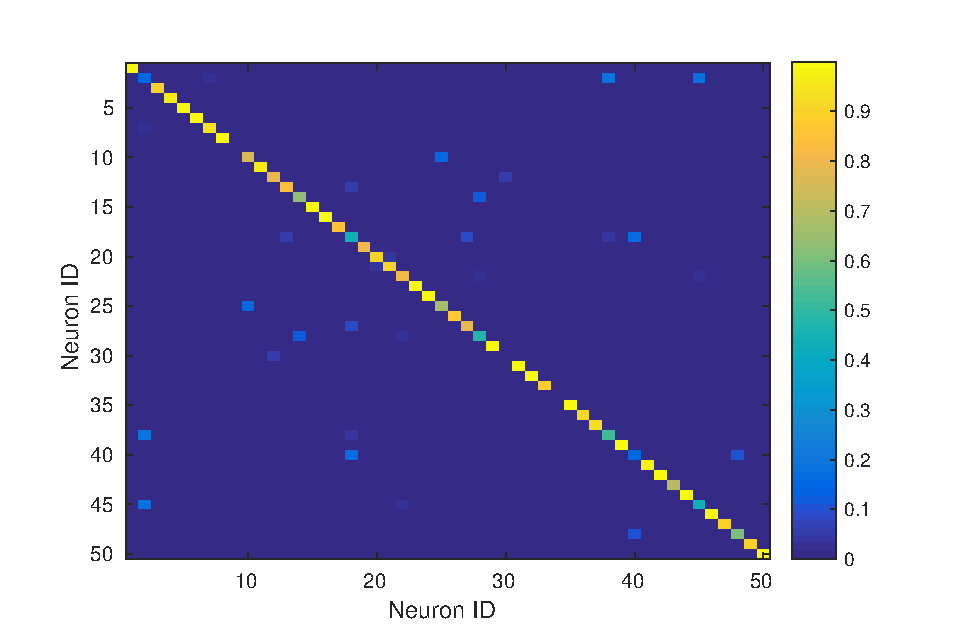
\includegraphics[width = \textwidth]{WW_6000Hz_Hebbian.eps}
\label{Compare: WW_Hebbian}
\caption{Multiplied weight matrix with Hebbian learning}
\end{subfigure}
\,
\begin{subfigure}[b]{0.49\textwidth}
\includegraphics[width = \textwidth]{WW_6000Hz.eps}
\label{Compare: WW_STDP}
\caption{Multiplied weight matrix with STDP learning}
\end{subfigure}
\\
\begin{subfigure}[b]{0.49\textwidth}
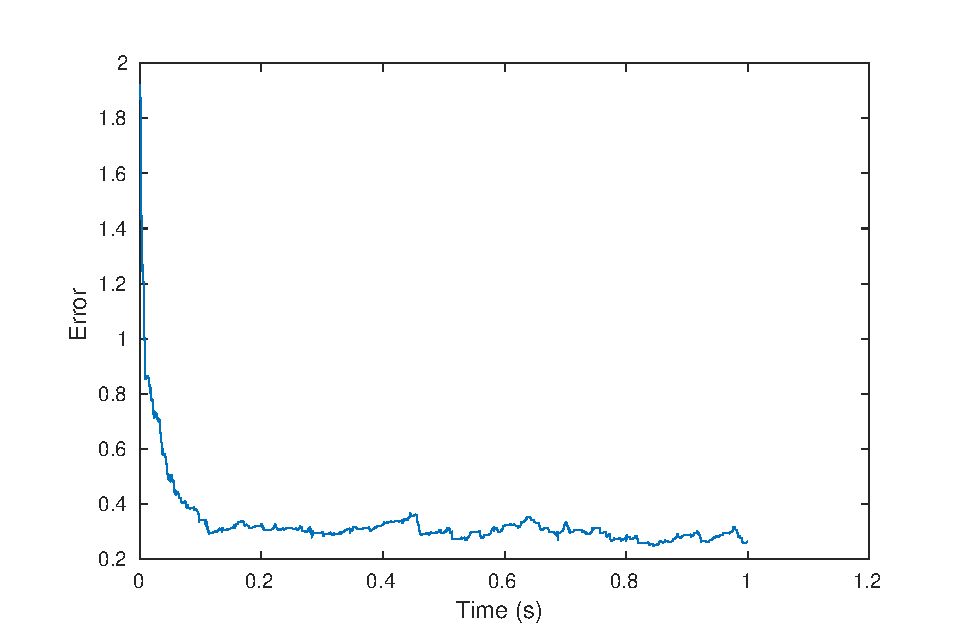
\includegraphics[width = \textwidth]{ErrorOverTime_6000Hz_Hebbian.eps}
\label{Compare: EoT_Hebbian}
\caption{Error over time of Hebbian plot}
\end{subfigure}
\,
\begin{subfigure}[b]{0.49\textwidth}
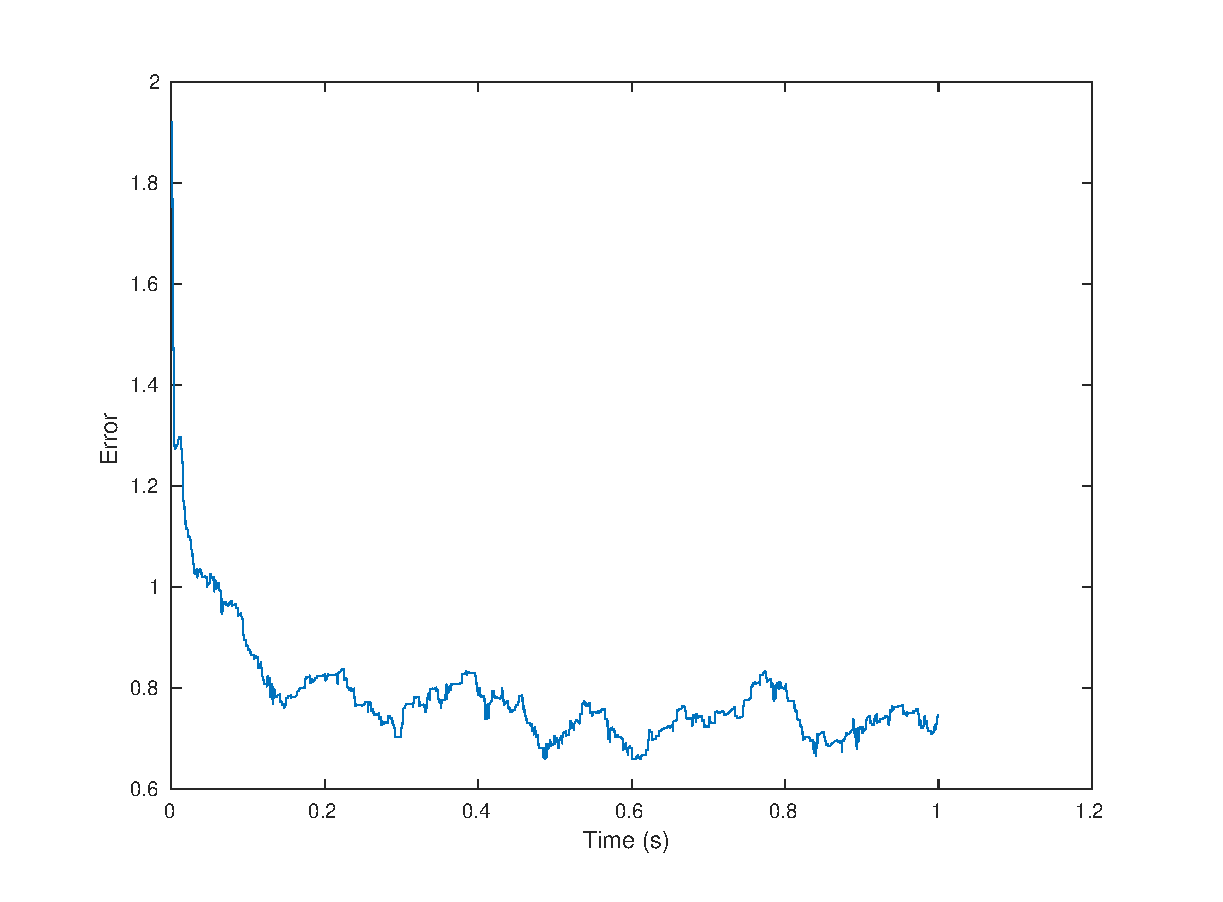
\includegraphics[width = \textwidth]{ErrorOverTime_6000Hz_normal.eps}
\label{Compare: EoT_STDP}
\caption{Error over time of STDP plot}
\end{subfigure}
\\
\begin{subfigure}[b]{0.49\textwidth}
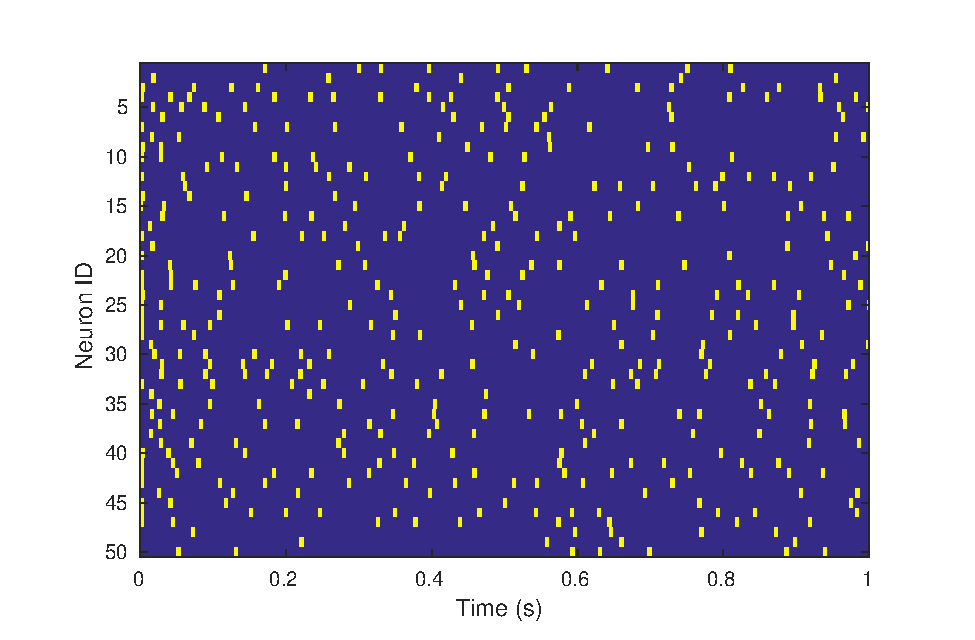
\includegraphics[width = \textwidth]{Burst_plot_6000Hz_Hebbian.eps}
\label{Compare: BH_Hebbian}
\caption{Burst history of Hebbian plot}
\end{subfigure}
\,
\begin{subfigure}[b]{0.49\textwidth}
\includegraphics[width = \textwidth]{Burst_plot_6000Hz.eps}
\label{Compare: BH_STDP}
\caption{Burst history of STDP plot}
\end{subfigure}
\label{Compare}
\caption{Compare STDP to Hebbian}
\end{figure}
\end{itemize}